\documentclass{article}
\usepackage{amssymb}
%% Language and font encodings
\usepackage[english]{babel}
\usepackage[utf8x]{inputenc}
\usepackage{times}

\usepackage{float}
\usepackage{subcaption}
\usepackage[rgb]{xcolor} % Needed by pdfcomment

\usepackage{import}
%% Sets page size and margins
\usepackage[top=1in,bottom=1in,left=1in,right=1in]{geometry}
\usepackage[labelsep=period]{caption}
%\renewcommand{\thetable}{\Roman{table}}
%% Useful packages
\usepackage{karnaugh-map}
\usepackage{tikz}
%\usepackage{amsmath}
\usepackage{url}
\usepackage{graphicx}
\usepackage[colorinlistoftodos]{todonotes}
\usepackage[colorlinks=true, allcolors=blue]{hyperref}
\floatstyle{plaintop}
\restylefloat{table}
\linespread{1.6}
\usepackage{epstopdf}
\epstopdfDeclareGraphicsRule{.tif}{png}{.png}{convert #1 \OutputFile}
\AppendGraphicsExtensions{.tif}
\setlength{\voffset}{0cm}
\setlength{\headsep}{0cm}
%\usepackage{amsmath} % or simply amstext
\newcommand{\angstrom}{\textup{\AA}}
\usepackage{siunitx}
\usepackage{array}% in the preamble
\usetikzlibrary{arrows,automata,positioning}
\newcolumntype{L}{>{\arraybackslash}m{7.25cm}}
\newcolumntype{C}{>{\centering\arraybackslash}m{3cm}}
\usepackage{enumitem}
\usepackage{listings}
\usepackage{xcolor}
 
\lstdefinestyle{customc}{
  belowcaptionskip=1\baselineskip,
  breaklines=true,
  frame=L,
  xleftmargin=\parindent,
  language=C,
  showstringspaces=false,
  basicstyle=\footnotesize\ttfamily,
  keywordstyle=\bfseries\color{green!40!black},
  commentstyle=\itshape\color{purple!40!black},
  identifierstyle=\color{blue},
  stringstyle=\color{orange},
}

\lstdefinestyle{customasm}{
  belowcaptionskip=1\baselineskip,
  frame=L,
  xleftmargin=\parindent,
  language=[x86masm]Assembler,
  basicstyle=\footnotesize\ttfamily,
  commentstyle=\itshape\color{purple!40!black},
}

\lstset{escapechar=@,style=customc}

\graphicspath{{images/}}
\usepackage{amsmath,amssymb}


\newcommand{\assignmentname}{ASSIGNMENT}
\newcommand{\HRule}[1]{\rule{\linewidth}{#1}}

\makeatletter

\renewcommand{\maketitle}{
\begin{titlepage}
\begin{center}
\textbf{\LARGE{ \huge \\ [4.0cm] \@title \\[0.3cm] \assignmentname}}
\HRule{2pt}
\LARGE{\textit{ \@author \\ [3.0cm]}
ECE 445 -- Spring 2020}
\end{center}
\end{titlepage}
}\makeatother

%%%%%%%%%%%%%%%%%%%%%%%%%%%%%%%%%%%%%%%%%%%%%%%%%

% Authors: Add additional packages and new commands here.  
% Limit your use of new commands and special formatting.

% Place your title below. Use Title Capitalization.


% Add author information below. Communicating author is indicated by an asterisk, the affiliation is shown by superscripted lower case letter if several affiliations need to be noted.

\title{Low-Cost Integrated Spectrometer}
\date{ Spring 2020 } % this is the name of the assignment
\author{
Group: 18 --\\ \textbf{Lukas Janavicius}: Physical Design, R\&V, Block Diagram \\ \textbf{Drew Ingram}: High-level, Visual Aid, Schedule\\ \textbf{Stephen Gioja}: Cost, Safety and Ethics \\[2.0cm]
NetIds: janavic2, andrewi2, and sgioja2\\
TA: Charles Ross
}




\newcommand{\Verify}[1]{
\item  #1 
}

\newcommand{\Verification}[1]{
\item
\begin{enumerate}\itemsep0em  #1\end{enumerate}
}

\newcommand{\Require}[1]{
\item  #1 
}

\newcommand{\Requirement}[2]{
\begin{table}[H]
\centering
\resizebox{\textwidth}{!}{%
\begin{tabular}{|L|L|}
\hline
\textbf{Requirement} & \textbf{Verification} \\ \hline
 #1  & \begin{enumerate}[label=(\alph*)] \itemsep0em  #2 \end{enumerate}       \\ \hline
\end{tabular}%
}
\end{table}
}

\newcommand{\Requirements}[2]{
\begin{table}[H]
\centering
\resizebox{\textwidth}{!}{%
\begin{tabular}{|L|L|}
\hline
\textbf{Requirements} & \textbf{Verification} \\ \hline
\begin{enumerate} #1  \end{enumerate}    & \begin{enumerate} \itemsep0em  #2\end{enumerate} \\ \hline
\end{tabular}%
}
\end{table}
}



% Cite documents by typing  \cite{ }
% Once that's up, you should see a list of really long names
% try searching by title, subject, or author

% Change this to whatever the assignment name is
\renewcommand{\assignmentname}{Design Document Check}


\begin{document}
\maketitle


\tableofcontents

\section{Introduction}

    \subsection{Objective}
    For three centuries, optical spectrometers have played instrumental roles in advancing nearly all branches of science, from discovering new elements, determining the composition of stars, or even identifying and characterization of Two-Dimensional materials \cite{Weeks1932TheDiscoveries, Loewen1997DiffractionApplications, WhatSpectroscopy}. Given the technology's maturity, modern-day spectrometers have evolved since their initial conception, collecting and quantifying their data for instant analysis. However, budget digital spectrometers, including their required software, start at over \$1000 \cite{OceanSpectrometers}. This cost barrier effectively limits spectrometry techniques to controlled laboratory environments in Universities and other research institutions. 
    
    We aim to bring the cost of the digital optical spectrometer, lowering the barrier of entry and extending the applications of spectrometry. A spectrometer's cost lies in its expensive optics and dedicated high-frequency data collection hardware. Our proposed solution is to eliminate costly optical components by integrating an optical circuit in acrylic plastic and collecting the diffracted light using a linear CCD image sensor driven by a low-cost microcontroller.
     
     
    \subsection{Background}
        Integrated Photonic Spectrometers (IPSs) are a well-studied subject, fabricated in various materials and geometries; however, such literature presents narrow and novel applications of the IPS like broadband single-photon spectrometers, while commercial devices start at over \$350 for the sensor alone \cite{Ma2013, Pottier2014IntegratedInsulator, Cheng2019BroadbandSpectrometer, BO-HAMA-2-C12880MADigiKey}. Additionally, several open-source projects demonstrate digital spectrometers built with the Arduino framework but are limited in that capturing a single data frame takes 4 seconds over the 8-bit microcontroller's 115.2 Kbaud USB-UART connection \cite{CCDAllmon}.
   

    \subsection{High-Level Requirements}
        \begin{itemize}
            \item The spectrometer's optics should be capable of resolving the plasma emission spectra of common gasses, such as argon.
            \item The spectrometer must be capable of live plotting and capturing data with a refresh rate of at least 10 hz.
            \item We must present a novel fabrication technique for a PMMA-based spectrometer to enable manufacturing at a significantly lower cost than current alternatives.
        \end{itemize}
       \begin{figure}[H]
       
    \centering
    \def\svgwidth{0.8 \columnwidth}
    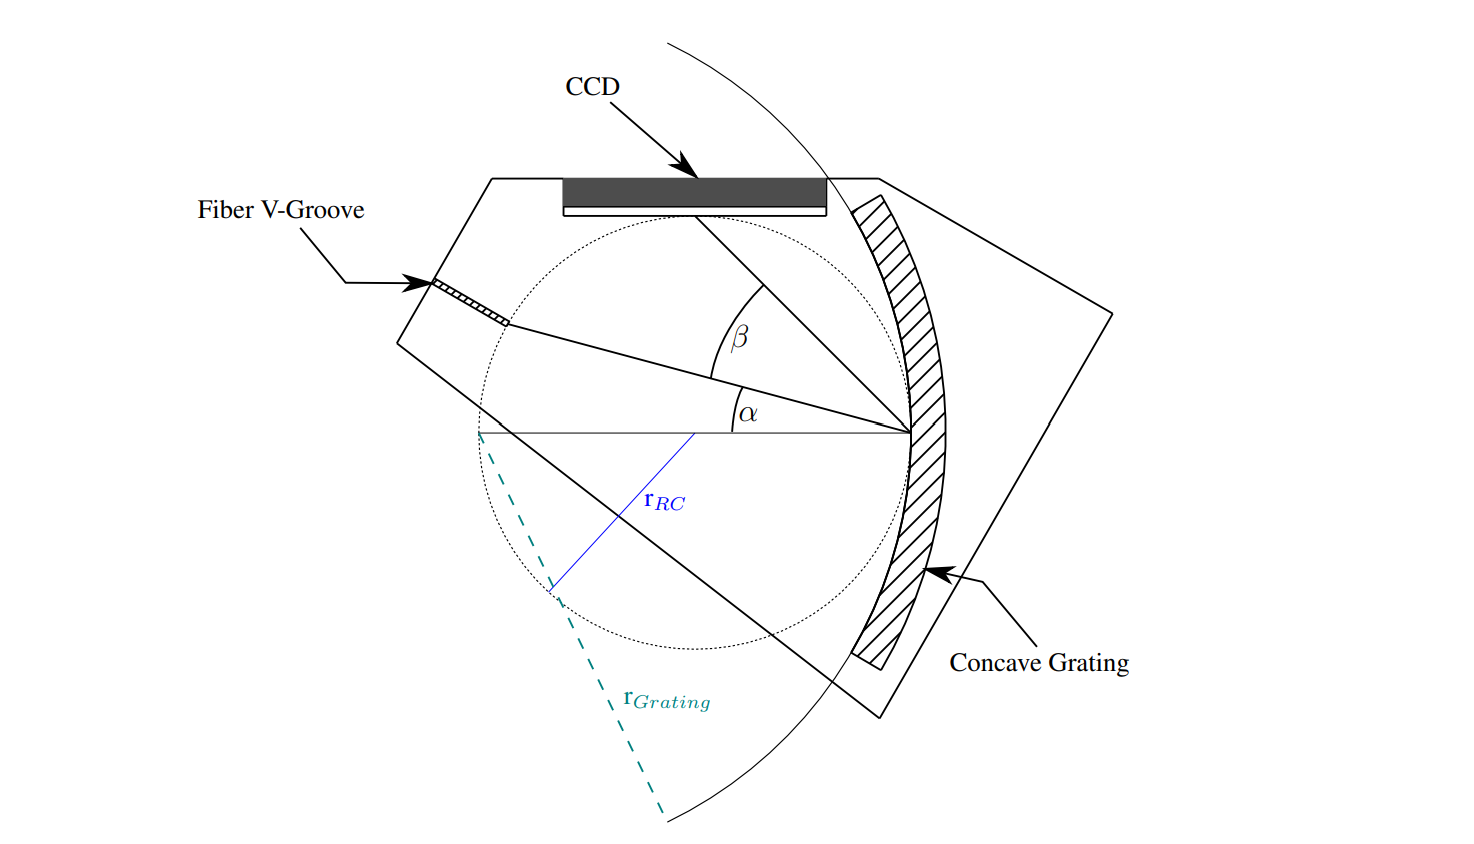
\includegraphics{images/grating_diagram_dd.png}
    %\includegraphics{images/proposal_layout.png}
    \caption{\label{fig:spec_intro}Spectrometer grating configuration. The grating lies on a circle of radius $r_{Grating} = 2 r_{RC}$, which is tangent to the Rowland Circle. The Rowland pole is the tangent point between these two circles, angles are defined from the line normal to the pole}
    \end{figure}
    

\section{Design}
    \subsection{Physical Design}
    Figure \ref{fig:physical}, The physical design of the spectrometer isolates the light sensitive hardware from the environment. Additionally, the optical feedthrough allows our spectrometer to connect to external optical fibers and instruments. The photonics are located off-center to allow for the ESP chip and its accompanying electronics. Also shown is the photonic slab mounted to the CCD. Figure \ref{fig:slablayout} shows the photonics package relative to the CCD. Angular measurements follow the work of P. Pottier and M. Packirisamy, while other dimensions are maximized to accommodate the package \cite{Packirisamy2013DesignMirrors}.
    
      The spectrometer design in Figure \ref{fig:block_diagram} requires three primary modules to fulfill the above requirements. The photonics demodulate light inbound through a coupled optical fiber, as in Figure \ref{fig:spec_dia} and the outbound light is coupled into waveguides carrying a given spectral band. By using a three-dollar microcontroller, the ESP32, we satisfy the remaining requirements, as it overcomes the communication bottleneck of the Arduino's USB-UART connection through WiFi. Additionally, with its two 240 MHz cores, the tasks of data acquisition and serving data to the user are split amongst the cores.
    
    \begin{figure}[H]
    \centering
    \scriptsize  
    \def\svgwidth{\columnwidth}
    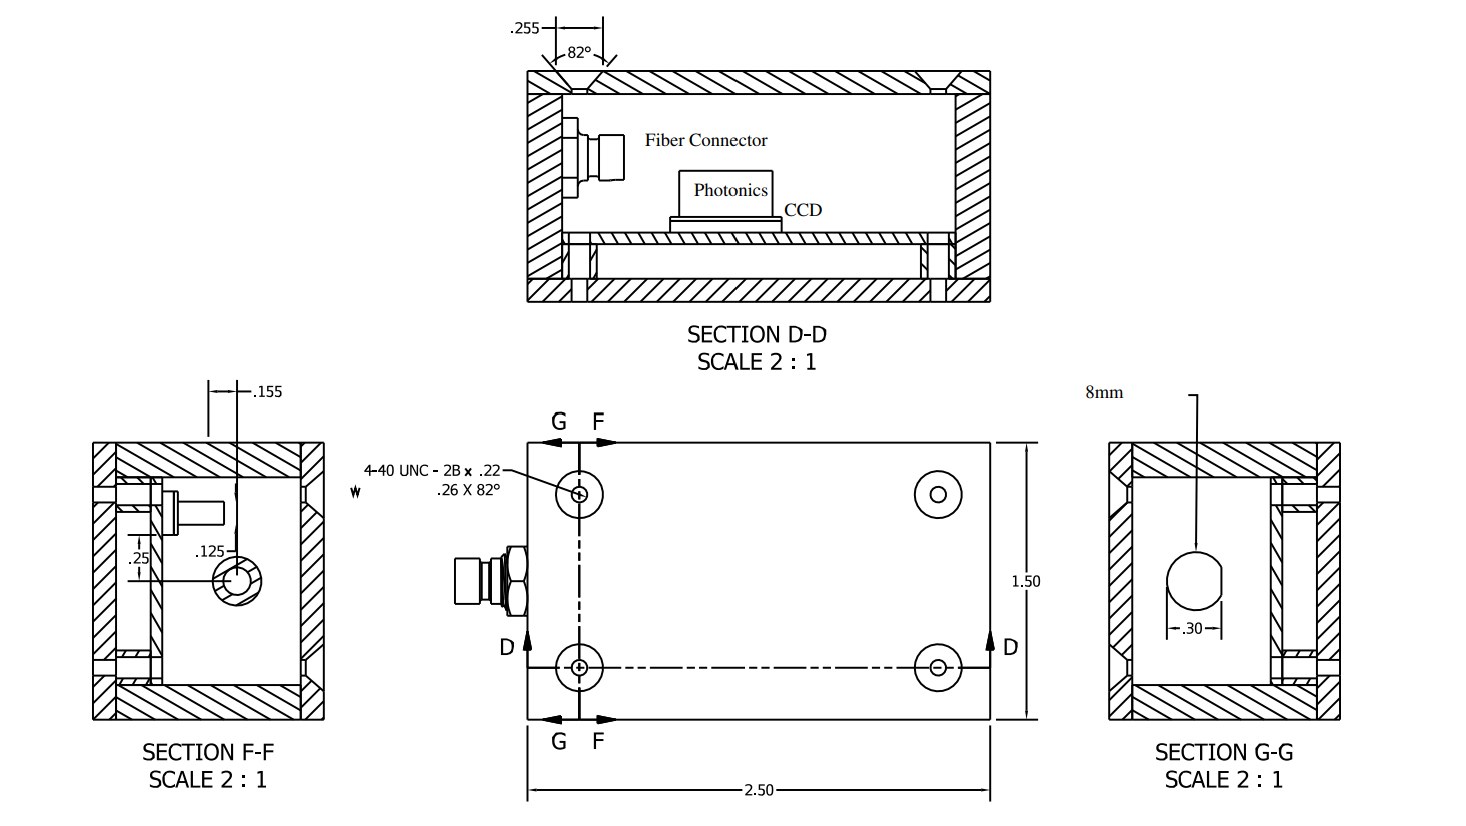
\includegraphics{images/proposal_physical.png}
    %\includegraphics{images/proposal_layout.png}
    \caption{\label{fig:physical}Spectrometer housing.}
    \end{figure}
    
    \begin{figure}[H]
    \centering
    \large
    \def\svgwidth{\columnwidth}
    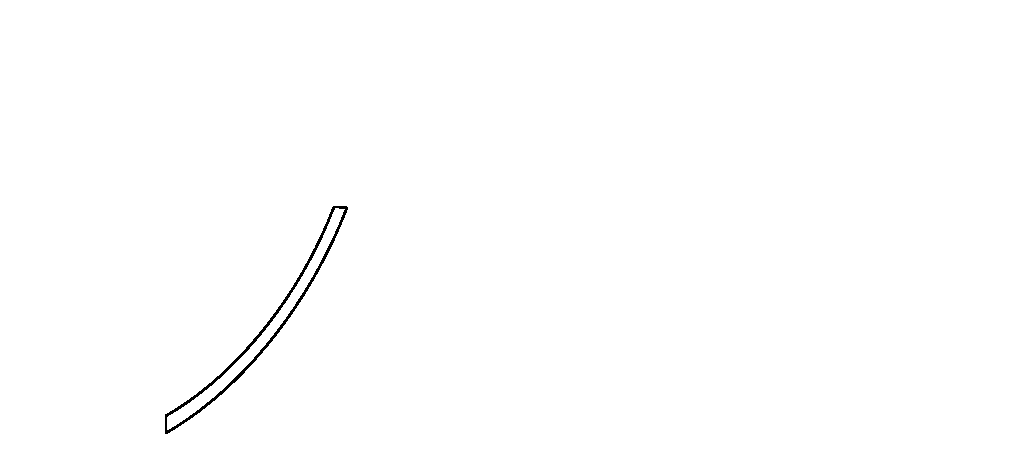
\includegraphics{"images/photonics layout.png"}
    %\includegraphics{images/proposal_layout.png}
    \caption{\label{fig:slablayout}Photonics Schematic $\alpha = -15^{\circ}$, $\beta = -45^{\circ}$, and other dimensions scale to accommodate $r_{RC}$.}
    \end{figure}


  
    
    \begin{figure}[H]
    \centering
    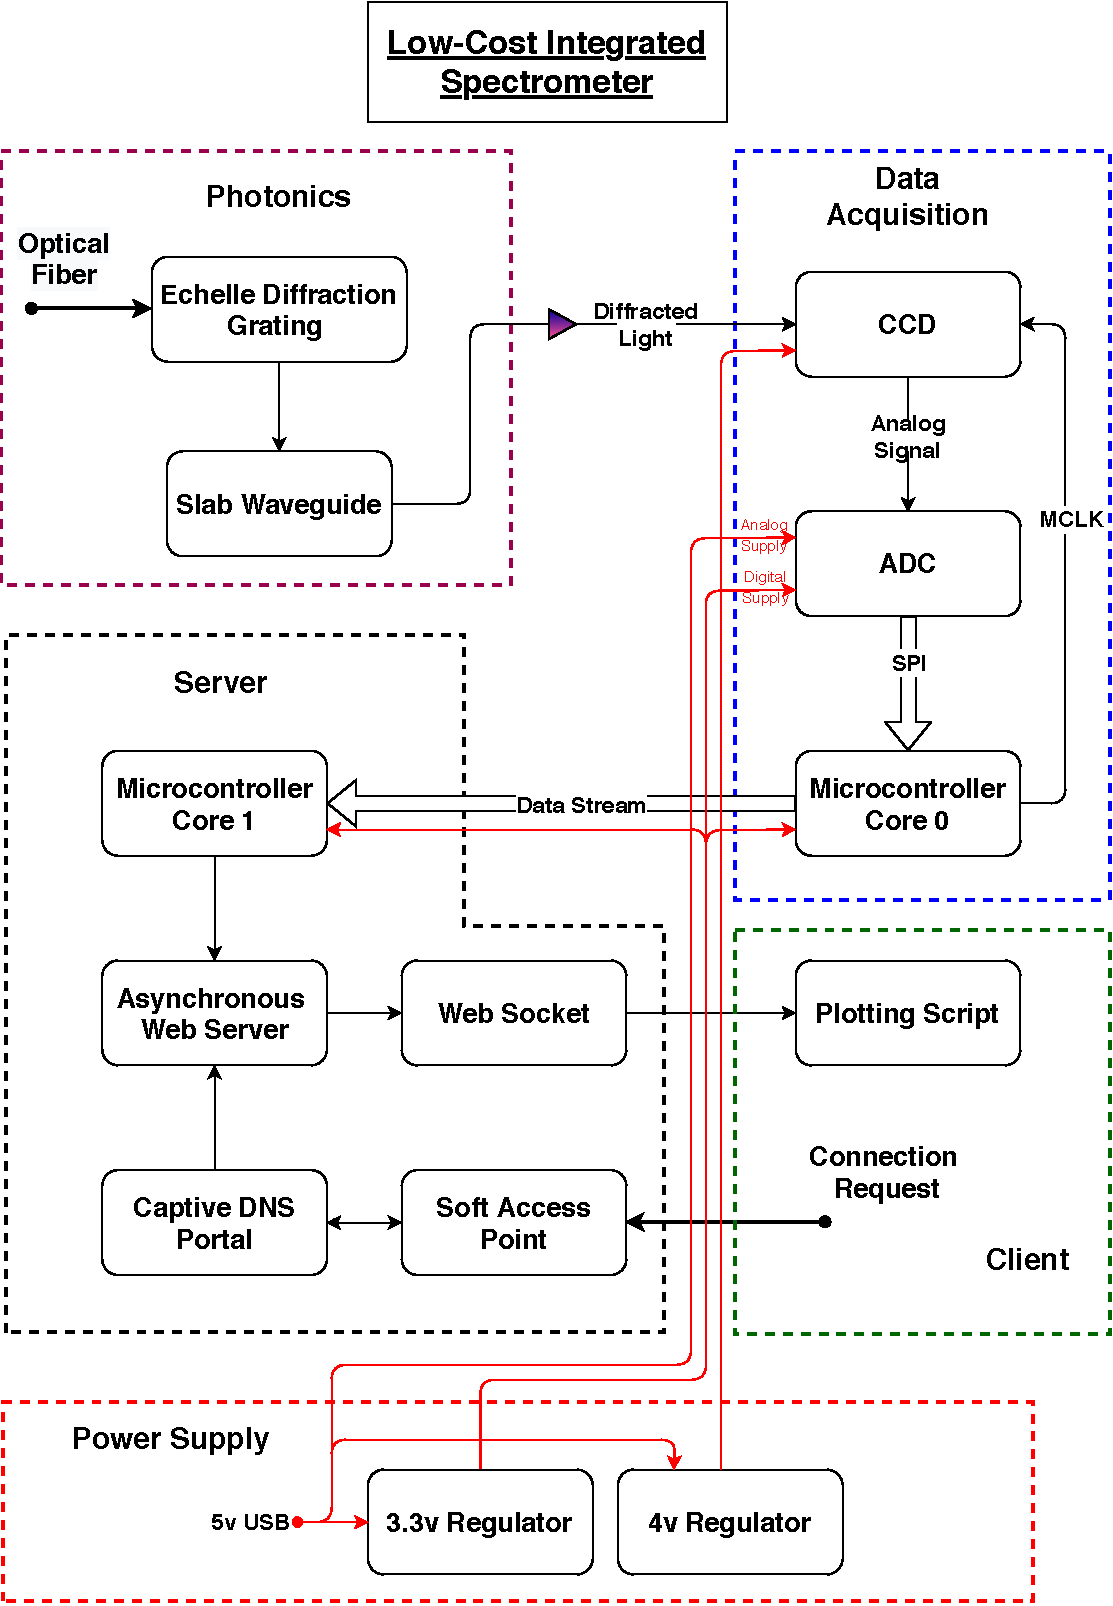
\includegraphics[width=0.8\textwidth]{images/Spectrometer Block Diagram.pdf}
    \caption{\label{fig:block_diagram}High-Level Block Diagram}
    \end{figure}
    
    \subsection{Photonics}
        \subsubsection{Concave Blazed Diffraction Grating}
        \begin{figure}[H]
        \centering
        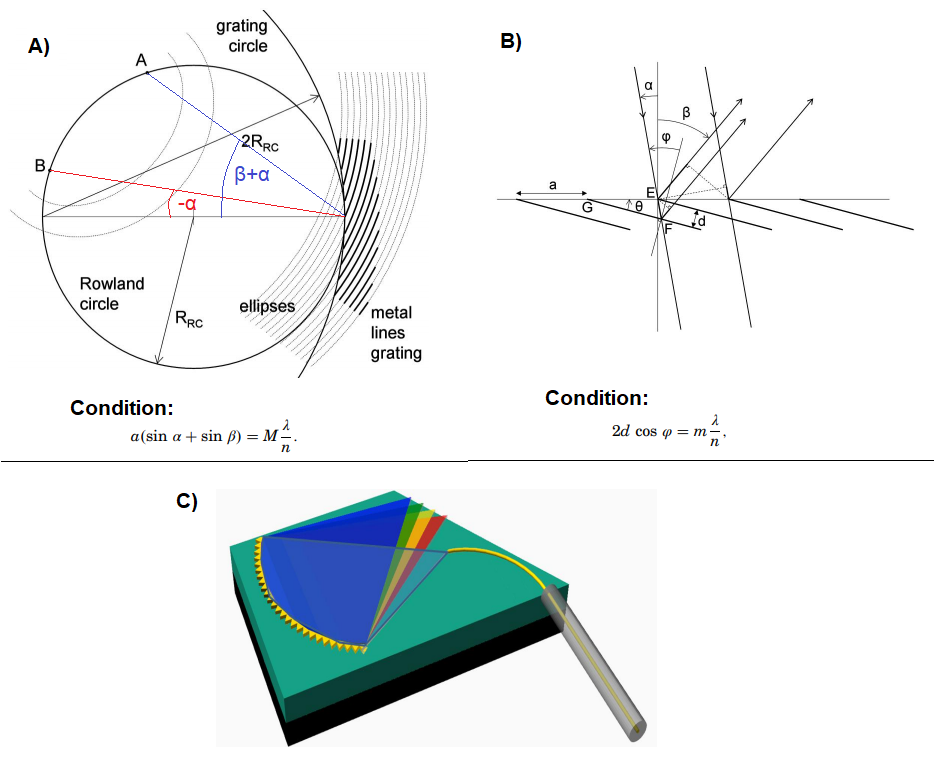
\includegraphics[width=0.8\textwidth]{images/gratingconditions.png}
        \caption{\label{fig:spec_dia}Integrated Spectrometer geometrical constraints from P. Pottier et al. \cite{Pottier2014IntegratedInsulator}. Subfigure A shows the general diffraction condition for a Rowland defined grating. Subfigure B shows the second, Bragg, diffraction condition of the elliptical grating. Subfigure C shows the device layout, the combined diffraction condition ensures only one output order \cite{Pottier2014IntegratedInsulator, Wang2019IntegratedAstronomy}}
        \end{figure}
        
        Different wavelengths of light will need to be physically separated. We plan to accomplish this by using an Concave Blazed grating, as in Figure \ref{fig:spec_dia}. Our design's constraints demand a larger feature size than that of detailed by P Potter et al, since MNTL's Heidelberg mla150 has a feature size of 600 nm.
        
        Equation \ref{eq:rowlandcond} describes the general diffraction condition for the Rowland mounted grating; $\lambda_{blazing} = 600$ nm is the center wavelength for our detection band, $M$ is the diffraction order, $\eta_{eff} = 1.5$, and $\sin{\alpha}$ and $\sin{\beta}$ are the input and output pole-angles respectively \cite{Packirisamy2012Mono-OrderGrating}. To meet the 600 nm feature size, $M \geq 2$, and in general a larger $M$ implies a larger device.
        
        \begin{equation}
           \begin{aligned}\label{eq:rowlandcond}
            a &(\sin{\alpha} + \sin{\beta})= M \frac{\lambda_{blazing}}{\eta_{eff}} \\
            a &= M \frac{\lambda_{blazing}}{\eta_{eff} (\sin{\alpha} + \sin{\beta})}
        \end{aligned}
        \end{equation}
     
        Equation \ref{eq:blazing} represents the blazing conditions of a two-material Distributed Bragg Reflector (DBR) system \cite{Packirisamy2012Mono-OrderGrating}. The chosen system is PMMA/air, $\eta_{eff} = 1.5$ and $\eta_{2} = 1$, which is identical to the index of refraction differential of Pottier et al. Equation \ref{eq:braggcond} describes the condition for the DBR's maximum reflectively, although such constraints can be relaxed if $d_2 \ll d$ \cite{Packirisamy2013DesignMirrors, Packirisamy2012Mono-OrderGrating}. 
        
        \begin{equation}
           \label{eq:blazing}
            d = -a \sin{\frac{\alpha + \beta}{2}} = d_1+d_2 
        \end{equation}
        
        \begin{equation}
           \begin{aligned}\label{eq:braggcond}
           \text{Given }\phi &= \frac{\alpha - \beta}{2} \text{, and } \eta_{eff} \sin{\phi} = \eta_{2} \sin{\phi_2}\\
            d1 &=  \frac{(2 k_1 +1) \lambda}{4 \eta_{eff} \cos{\phi}} \text{, where $ {k_1} \in \mathbb{Z}$} \\
            d2 &=  \frac{(2 k_2 +1) \lambda}{4 \eta_{2} \cos{\phi_2}} \text{, where $ {k_2} \in \mathbb{Z}$}
         \end{aligned}
        \end{equation}
        
        Equation \ref{eq:fsr} represents the Free Spectral Range (FSR), $\Delta \lambda$, or the maximum bandwidth of the detection region \cite{Mao2019PerfectPlatform}. For our system $\Delta \lambda \rvert_{M=2} = 525$ nm and $\Delta \lambda \rvert_{M=3} = 333$ nm, in general as the bandwidth goes down the resolving power of our grating goes up. With these parameters, we can tune the wavelength response band and resolution within that band.
        
        \begin{equation}\label{eq:fsr}
            \Delta \lambda = \frac{\lambda_{blazing}}{M}(1- \frac{M+1}{M}(1-\frac{\eta_{eff}}{\eta_{2}}))
        \end{equation}
        
        \begin{figure}[H]
        \centering
        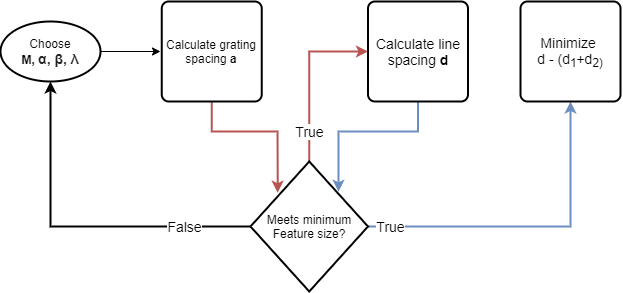
\includegraphics[width=0.8\textwidth]{images/grating_types.png}
        \caption{\label{fig:gratingflowchart}Diffraction Grating Design Flow-Chart}
        \end{figure}       
        
        \subsubsection{Slab Waveguide}
        An optical fiber must couple light into the acrylic. For this we propose a laser-engraved v-groove mounting, coupled via epoxy to an acrylic slab waveguide. The waveguide confines light within two dimensions and directs it to the CCD. Our fabrication should exceed a 10 micron etch depth to ensure multimodal transport.
        
        
    \subsection{Data Acquisition}
        \subsubsection{CCD}
       Detects and measures the intensity of light on each pixel. The array of pixels allows us to resolve the output spectrum spatially. The CCD integrates the output spectrum with time, to prevent overexposure, it must be refreshed at a high rate, 1-2 MSPS. We propose using the TCD1103GF from Toshiba for its standard interface, low-cost, and 3.3V compatibility.
        \textit{\\Requirement: Must drive the MCLK at 2-4 MHz. }
        
        \begin{figure}[H]
        \centering
        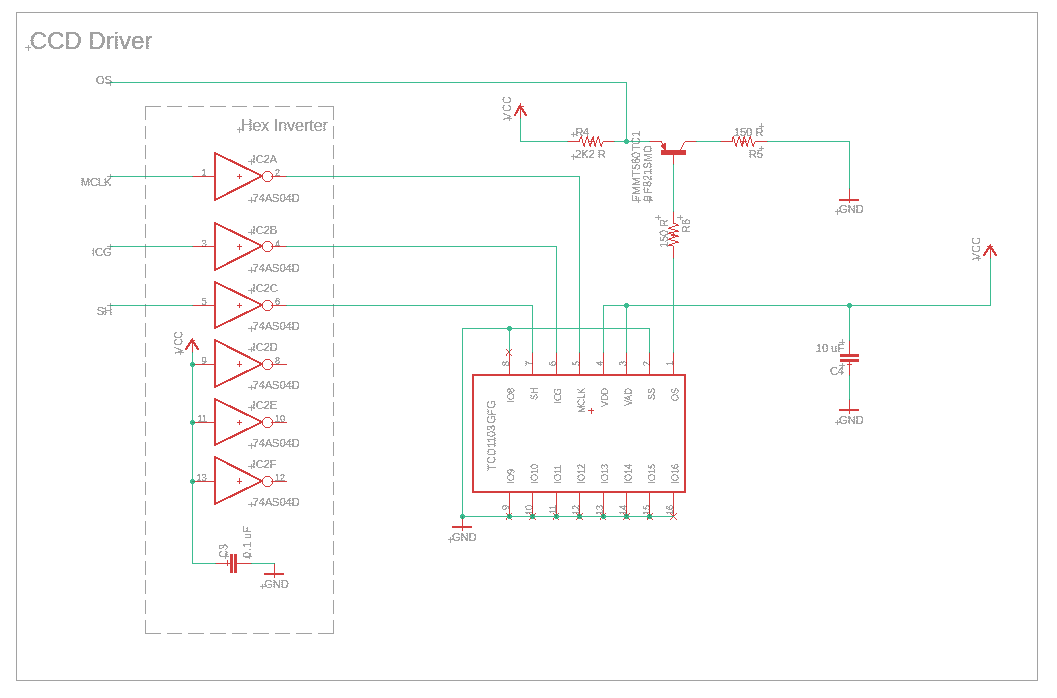
\includegraphics[width=0.8\textwidth]{images/ccdschem.PNG}
        \caption{\label{fig:ccdsc}CCD Driver Schematic}
        \end{figure}
        
        \subsubsection{ADC}
        The The ADC converts the CCD's analog readings to digital data for the ESP32. To match the CCD's speed the ADC must be compatible with the ESP's fastest serial communication standard SPI, and offer atleast 2 MSPS.
        
        \begin{figure}[H]
        \centering
        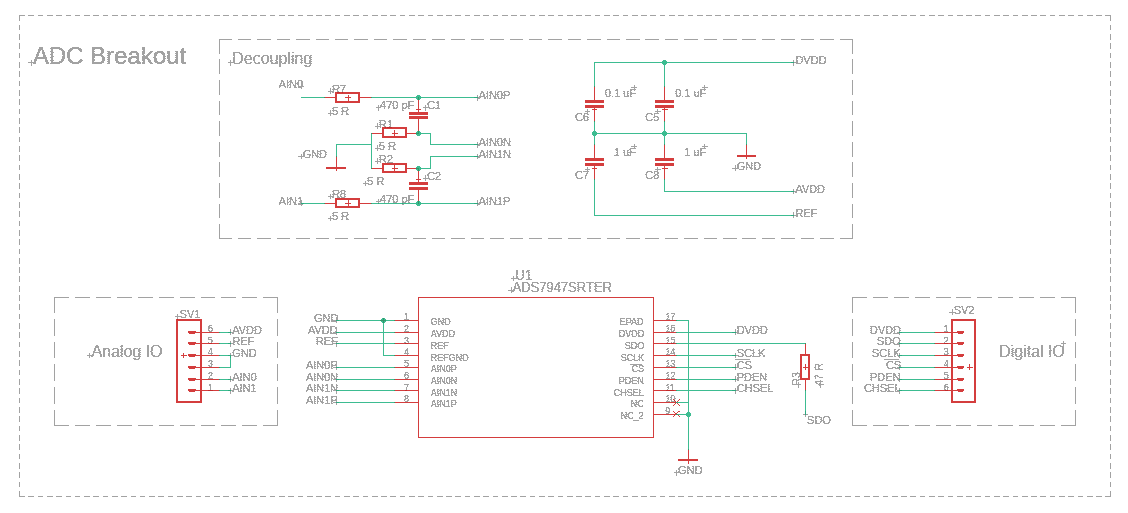
\includegraphics[width=0.8\textwidth]{images/adcschem.PNG}
        \caption{\label{fig:adcsc}ADC Device Schematic}
        \end{figure}
        
        \subsubsection{Microcontroller Core 0}
             At a high level, the ESP32 SOC is configured with two tasks. Initially, we configure the platform's 16 peripheral timers, capable of a maximum of 40 MHz, to generate the necessary clock signals signal. Then, the task of monitoring the board hardware communicates with the ADC over SPI. Incoming data is streamed to the second core, which hosts an asynchronous web server.
             
    
    \subsection{Server}
        The server will comprise an ESP32 hosting a network access point where the intended user can connect and log on to view their data in a web browser. The implementation of the server is beyond the scope of this class; however, the general requirements of each components are listed below.
        \subsubsection{Microcontroller Core 1}
            This Microcontroller asynchronously communicates to its WiFi IC and the other core. Additionally it hosts our web server with a complementary file-system.    
            \textit{\\Requirement: Cannot bottleneck the 10 frames-per-second required above.}

        \subsubsection{Asynchronous Web Server}
            \textit{Requirement: Must serve the plotting script, and establish a websocket connection.}
            
        \subsubsection{Web Socket}
            Connects to the user's plotting script to stream the spectrum's data. The async server host's the websocket, and connects the user to it.
            \textit{\\Requirement: Must connect to the user's plotting script and stream the data atleast 30kbps.}
            
        \subsubsection{Captive DNS Portal}
            \textit{Requirement: Must immediately forward anyone connecting to our network to a webpage with our plotting script.}
            
        \subsection{Soft Access Point}  
            \textit{Requirement: Must allow users to connect by joining the WiFi network.}
            
        \subsubsection{Plotting Script}
            \textit{Requirement: Defines a set of API functions which receive data from the microcontroller and forward them to a JavaScript plotting API \cite{ESP32/ESP8266Tutorials}}.
    
            
    \subsection{Risk Analysis}
    The most challenging component to design will likely be the photonic circuit. The diffraction grating's geometrical constraints have only been proven for a simple concave blazed grating, whose effieciency has been simulated at less than 39\% \cite{Packirisamy2013DesignMirrors, Packirisamy2012Mono-OrderGrating, Pottier2014IntegratedInsulator}. The same work demonstrates using Bragg reflectors to produce Mono-Order diffraction gratings at greater than 99\% efficiency. 
    
    The grating also challenges the fabrication process; we must maximize reflectively, while performing a high aspect ratio etch. We must tune our UV exposure and development time to reach our desired aspect ratio, and optimize our grating geometry. If the etch is not consistent throughout, our calculated path-length differences no longer hold and our grating will fail.
    


\section{Requirements and Verification}
\subsection{Diffraction Grating [40 Points]}

    \Requirement{ Must diffract light within the range of 400-800 nm
            } { \Verify{Place grating inside nanolab's quantum efficiency (QE) measurement system, between the Monochromator and CCD.}
                \Verify{Sweep input wavelengths across the specified range, record the output diffraction order's position on the CCD as a function of wavelength.}
                \Verify{Ensure our grating geometry supports a single high-order diffraction order, and that the output range falls within the detector length.}
                \Verify{Compare input and output optical power across full band to calculate efficiency}
                }
                
\subsection{Slab Waveguide [10 Points]}

\Requirement{ The slab's thickness must exceed 10 microns.
        } { \Verify{Record the time spent developing the diffraction grating.}
            \Verify{Depth measurements at this feature-size are possible with the nanolab's Keyence VWX microscope's 3D imaging.}
            \Verify{If etch depth is too shallow, increase development time.}
            }

\subsection{Data Acquisition [20 Points]}

\Requirement{  Must sample at a rate of 1-2 MSPS
                    } { 
                        \Verify{Establish SPI communication with the ADC}
                        \Verify{Generate a 0.5-1 MHZ sine wave with a function generator.}
                        \Verify{The data rate out of the CCD must be the same as the ADC, 1-2 MSPS, by the nyquist condition the ADC should reconstruct the signal.}
                        \Verify{Run SPI communication between ADC and CCD and ensure 10 Hz polling rate.}
                    }

\subsection{Microcontroller [30 Points]}

 \Requirements{ \Require{ Must generate multiple 1-4 MHz clock signals for driving the CCD}
                            \Require{ SPI communication must support atleast 10 full 1500-pixel frames each second (30kbps)}
                        } { 
                            \Verification{
                                \Verify{Configure the ESP to PWM 0-40 MHz on all clock related GPIO.}
                                \Verify{Confirm all clock pins can output atleast their respective maximum frequencies with an oscilloscope.}
                            } 
                             \Verification{
                                \Verify{Establish SPI communication with the ADC}
                                \Verify{Generate a 500 KHz sine wave with a function generator.}
                                \Verify{As before, if the microcontroller reconstructs the signal, the data-rate exceeds 30 Kbps.}
                                
                            }
                        }
                        

\section{Cost and Schedule}

\subsection{Cost Analysis}

We estimate the hourly rate at approximately \$42/hr using Engineering Illinois's calculated \$84,250 for the year 2014-2015. 
The number of hours each of us spend per week will vary throughout the semester, but we estimate 10hrs/wk average for the three of us and be able to complete the prototype design within the 16 week semester, Equation \ref{eq:cost1}
. Additionally, Equation \ref{eq:cost2}, we estimate our cleanroom costs using UIUC's MNTL hourly-rate for industry at \$75/hr. We assume two individuals will spend under 10 hours each weeks for 8 out of the 16 work weeks in the semester. 
\begin{equation}\label{eq:cost1}
    3 \times \frac{\$ 42}{\text{hr}}\times \frac{10 \text{hr}}{\text{wk}} \times  16 \text{wk}  \times  2.5 = \$50,400 
\end{equation}

\begin{equation}\label{eq:cost2}
     2 \times \frac{\$ 75}{\text{hr}}\times \frac{10\text{hr}}{\text{wk}} \times  8 \text{wk}  \times  2.5 = \$30,000
\end{equation}

Our parts and prototype creation costs are estimated to be \$2.98 per unit.

\begin{center}
\begin{tabular}{ |l|r| } 
 \hline
 Part & Cost \\ 
 \hline
 ESP32 dual core microcontroller breakout board (mouser) & \$10.00  \\ 
 TI Analog to Digital converter ADS7947SRTER (mouser) & \$3.59  \\ 
 Toshiba CCD Linear Image Sensor TCD1103GFG (mouser) & \$14.79  \\ 
 Assorted Resistors, Capacitors, ICs, Sockets & \$10.00  \\
 PCB (PCBWay) & \$4.60 \\
 \hline
 Total & \$42.98 \\
 \hline
\end{tabular}
\end{center}

We plan to build 5 prototypes with a total production cost of \$92,614.90.

\subsection{Schedule}
    \begin{figure}[H]
    \centering
    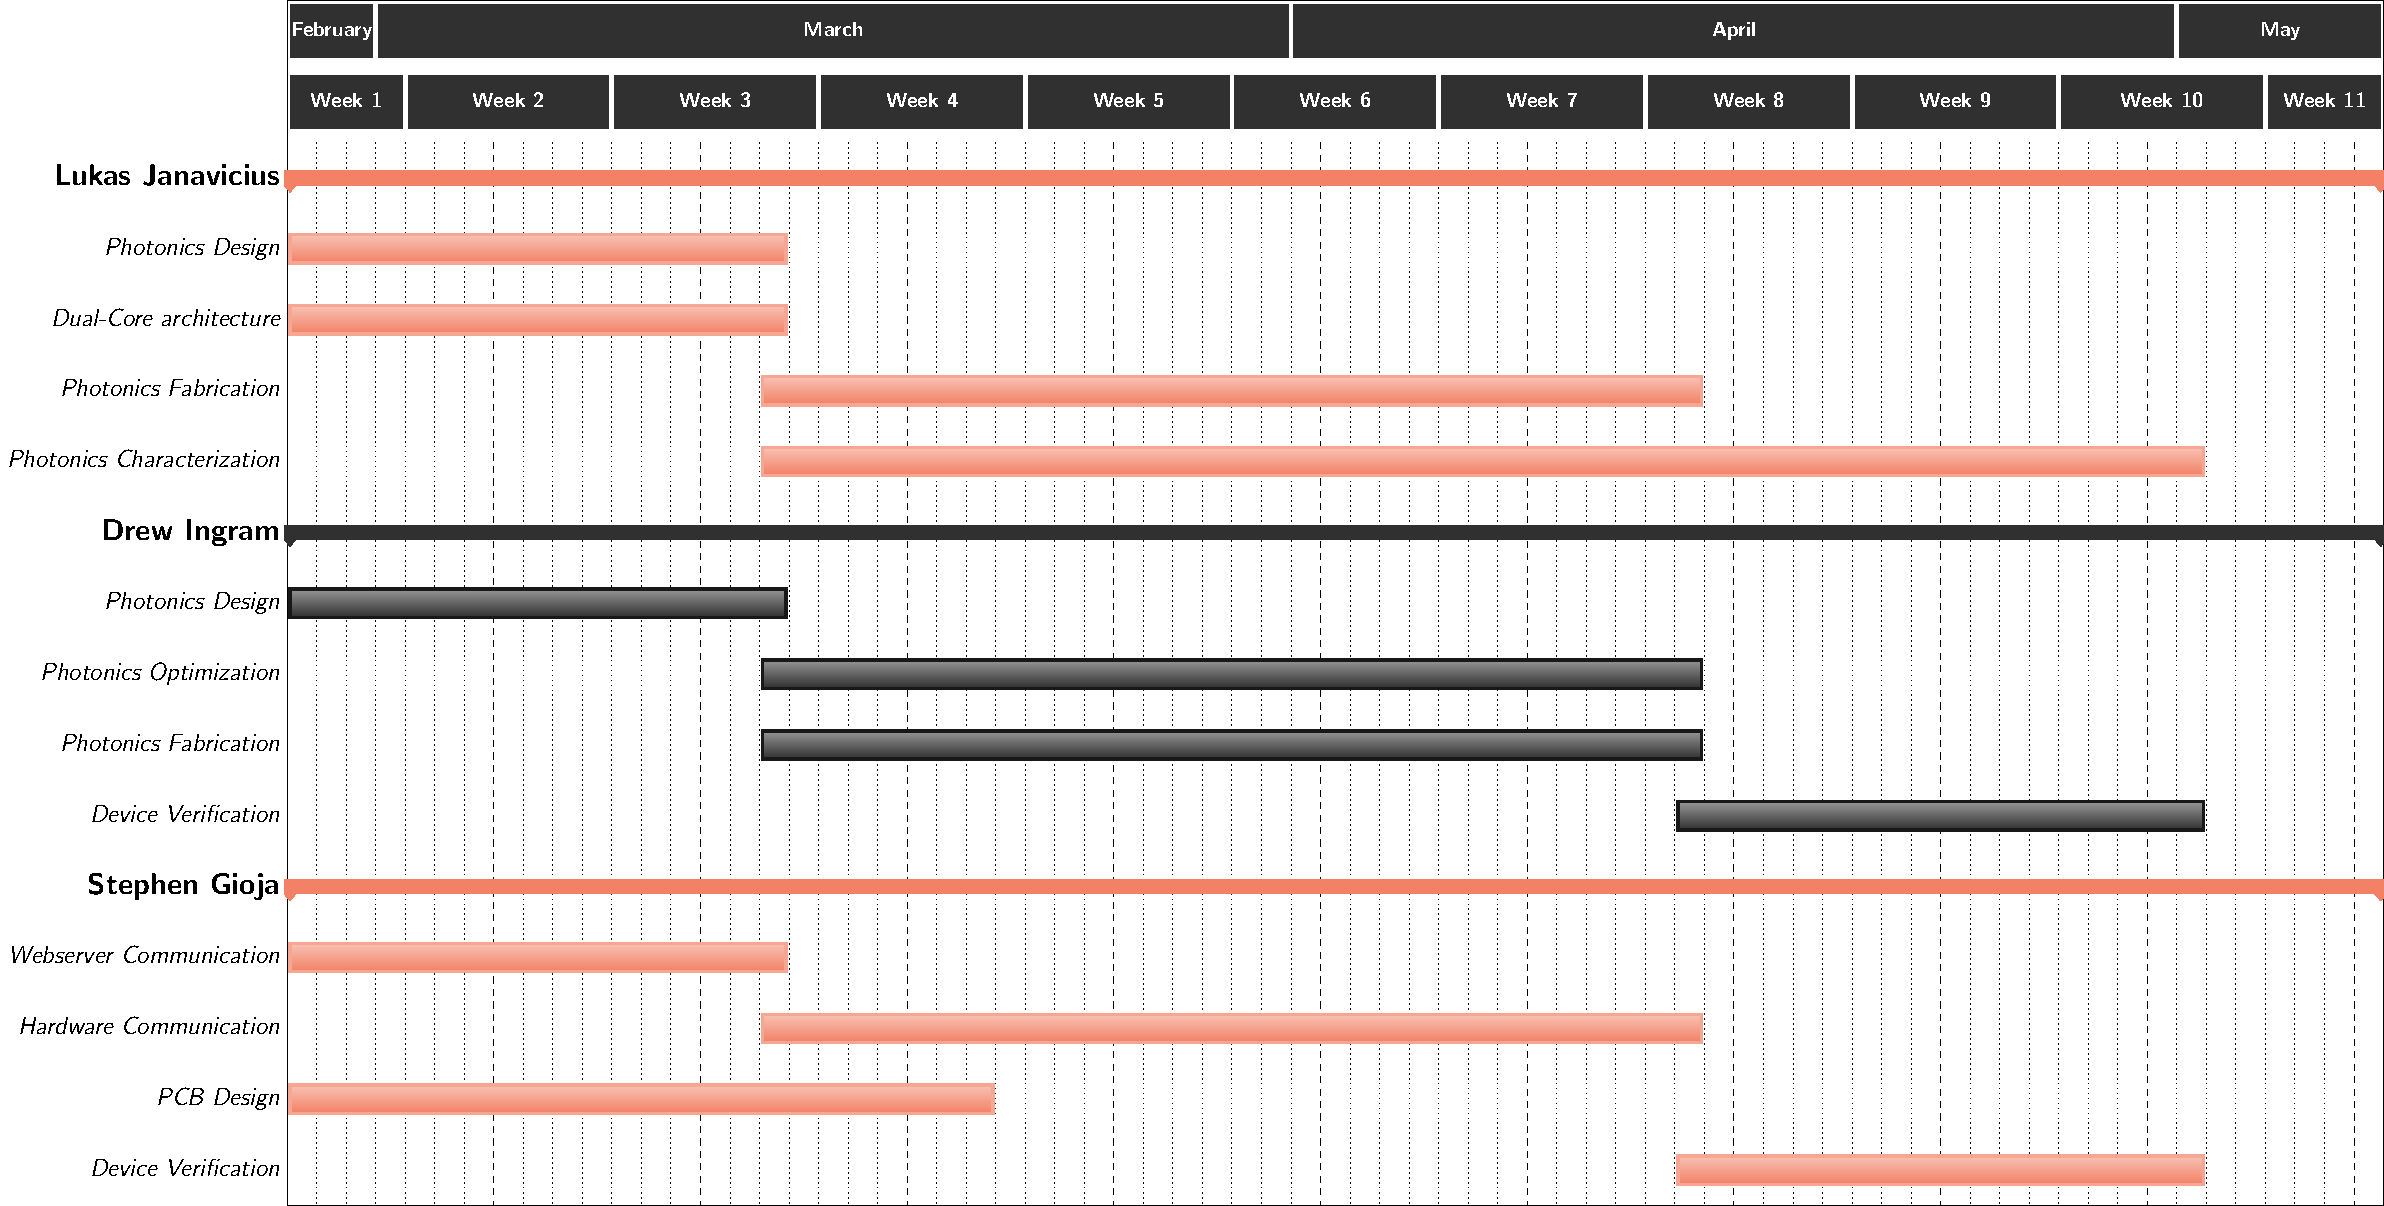
\includegraphics[width=\textwidth]{images/senior_design_schedule.pdf}
    \caption{\label{fig:schedule}Project Schedule.}
    \end{figure}
\section{Safety and Ethics}

In the ACM Code of Conduct section 3.1 we see the main point of designing a new or enhanced device is should be to improve the lives of people \cite{ACMConduct}. This is our main goal which is reached by decreasing the cost of a spectrometer and therefore increasing the ability for people to obtain one. This would have a positive impact on scientific education from grade school to university.

We recognize that our device will handle data belonging to its users. Data from our device could potentially be used in scientific research and other sensitive applications. The user's data must remain private to the intended users \cite{ACMConduct}. Our device will host a private network access point. Unauthorized users could potentially log in and access someone's data or cause data loss. We will mitigate these issues by presenting the users with a standard network login using password protection.

While developing we must respect the works of others, which includes citing our sources and not claiming the works of others as our own seen in Section 1.5 of the ACM Code of Ethics \cite{ACMConduct}. Section 2.4 of the ACM Code discusses giving/receiving feedback. We must listen to the feedback from our instructors and TA's and consider it in our design.                        
                        
                        
\clearpage
\newpage
\bibliographystyle{IEEEtran}
\bibliography{bibliography/references}
\end{document}
